\section{Materiales y métodos} \label{materiales_metodos}

\subsection{Flujo de trabajo}

Un cliente de escritorio se comunica con el dispositivo a través de un cable USB (\textit{Universal Serial Bus}
), que proporciona el medio físico para establecer un protocolo de comunicación UART (
\textit{Universal Asynchronous Receiver-Transmitter}
). Esta utiliza como broker a un proceso que se comunica con el microcontrolador y reproduce los estímulos sonoros a
través de terminales aéreos u óseos que se conecten al ordenador. Para una descripción más detallada del código
utilizado, se recomienda consultar el repositorio del trabajo, el cual se encuentra en GitHub (ver Anexo).

Dentro del dispositivo, un microcontrolador ESP32 \cite{espressif-systems-ESP32}
se emplea para muestrear y cuantizar la señal analógica, al mismo tiempo que transmite los datos recibidos al cliente de
escritorio. La señal analógica es adquirida y preacondicionada por una placa impresa (PCB, de
\textit{Printed Circuit Board}) construida para este propósito.

Como ordenador se empleó una Laptop HP Envy x360 2022 con Windows 11. Utilizar el mismo dispositivo en cada prueba
permite asegurar reproducibilidad en los niveles auditivos y las latencias en la transmisión de datos y reproducción de
estímulos auditivos. Si se utiliza un ordenador u audífonos diferentes, se recomienda recalibrar las amplitudes sonoras.

\subsection{Placa de preacondicionamiento}

Como se explicó anteriormente, la señal de interés debe ser amplificada en una etapa previa a su digitalización. Para
lograr esto realizamos una PCB que fue diseñada en Kicad \cite{kicad}. El circuito (Figura
\ref{fig:preconditioning-board-schematic}
) tiene como entrada un puerto jack de 3.5mm en el que se puede conectar los electrodos. Esos tres electrodos consisten
en entrada positiva, entrada negativa y voltaje de referencia (\textit{Vref}
). A continuación, los terminales se conectan a una etapa de preamplificación otorgada por un AD620, que obtiene la
diferencia de la entrada positiva y negativa, al mismo tiempo que elimina el ruido de modo común. Se amplifica con una
ganancia de 50.4, empleando una resistencia de 1 k$\Omega$
, de acuerdo a lo estipulado con la ecuación de ganancia en su hoja de especificaciones \cite{analog-devices-no-date}.

\begin{equation}
    G_1 = \left(\frac{49.4 \, \text{k}\Omega}{1 \, \text{k}\Omega}\right) + 1 = 50.4
    \label{eq:gain_calculation_1}
\end{equation}

\begin{figure}[H]
    \centering
    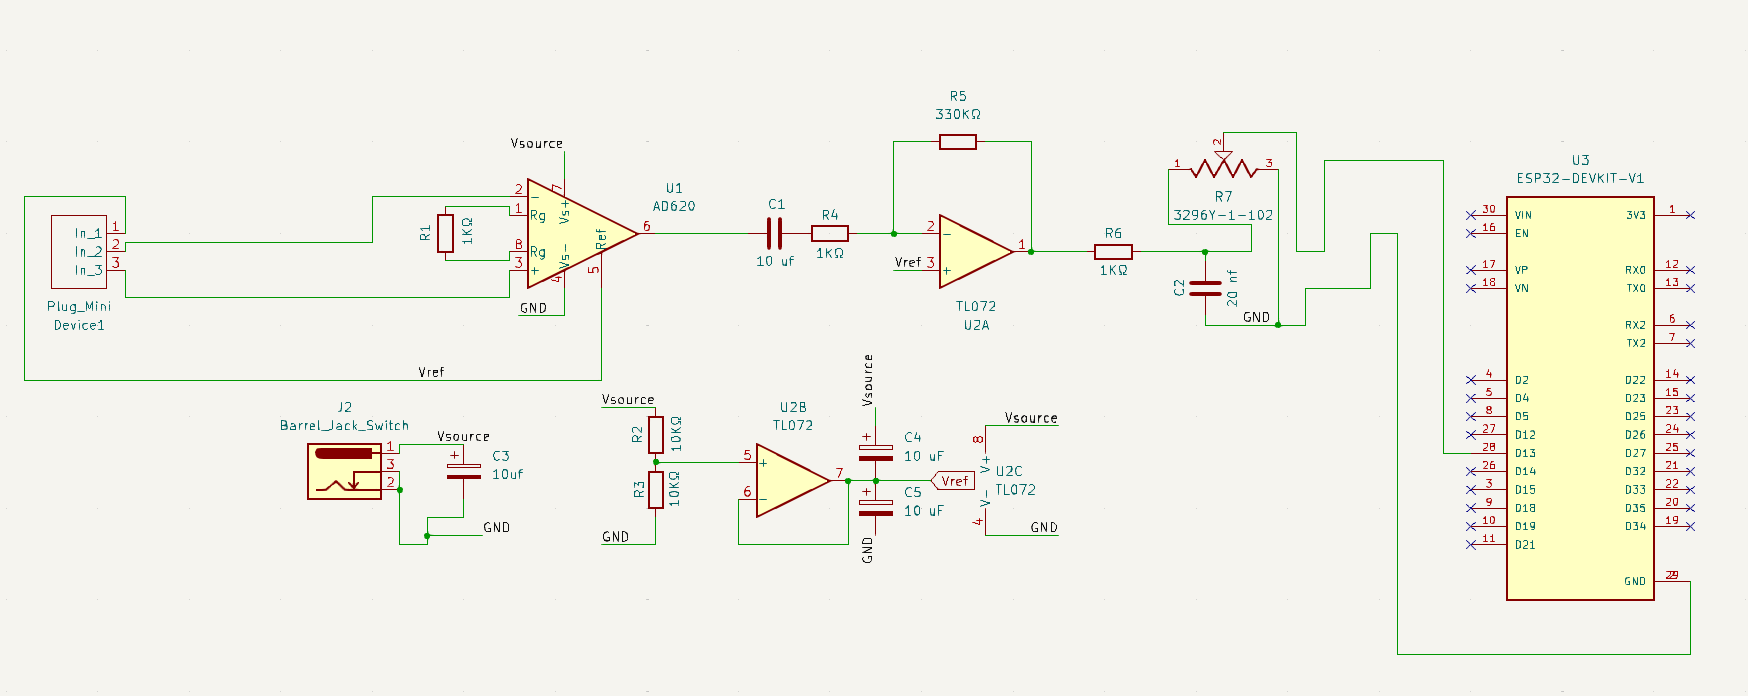
\includegraphics[width=1\linewidth]{figuras/Esquematico-Kicad.png}
    \caption{Esquemático de la placa de preacondicionamiento.}
    \label{fig:preconditioning-board-schematic}
\end{figure}

La salida del amplificador de instrumentación pasa a un filtro de desacople de continua formado por un operacional en
configuración inversora. La impedancia de entrada está compuesta de un capacitor de 10$\mu$
F en serie con una resistencia de 1 k$\Omega$, y la impedancia de retroalimentación es una resistencia de 330 k$\Omega$
. El amplificador operacional utilizado es el TL072. La transferencia de esta etapa es la siguiente:

\begin{equation}
    H_2 =  -\frac{Z_O}{Z_I} = -\frac{R_O}{R_I + \frac{1}{2 \pi j f C_I}} = - \frac{R_O}{R_I}
    \frac{1}{1 + \frac{1}{2 \pi j f R_I C_I}}
    \label{eq:gain_calculation_2}
\end{equation}

Por lo que obtenemos una ganancia (absoluta) de 330, con una frecuencia de corte de alrededor de 16Hz.

Luego esta señal es filtrada por un filtro pasabajos \textit{antialiasing} con una resistencia 1 K$\Omega$
y un capacitor de 20 nF para tener una frecuencia de de corte cerca de 8kHz.

\begin{equation}
    f_{c_{LP}} =\frac{1} {2\pi \left(1 \times 10^{3}\Omega \right) \left(20 \times 10^{-9}\mu F \right) } = 7.96kHz
    \label{eq:low_pass_cutoff}
\end{equation}

No se realizó un filtro pasabajos antialias con alto rendimiento debido a que la frecuencia de muestreo de la señal
adquirida (16kHz) es alta dentro del contexto de señales biológicas y la potencia del EEG disminuye notoriamente luego
de los 500Hz \cite{encyclopedia-scholarly-community}.

Finalmente, se encuentra un potenciómetro que fue calibrado de tal forma que garantice que la señal que llega al
microcontrolador no exceda los 3.2V, límite máximo para el ADC (\textit{Analog-to-Digital Converter}
) cuando este es configurado con atenuación máxima. Dado que la alimentación de la placa tiene una cota superior en 8V,
este potenciómetro reduce la ganancia efectiva en un 60\%
, dando como resultado una ganancia global de aproximadamente 6.7k.

\begin{equation}
    G_T = 0.4 G_1 G_2 = 0.4 \times 50.4 \times 330 = 6653
\end{equation}

La alimentación de los componentes activos se realiza utilizando dos pilas de 3,7 volts en serie (\textit{Vsource}
) que se conectan por un barril hembra a la placa de preprocesamiento. Con dos resistencias de 10 k$\Omega$
, se logra un divisor resistivo simétrico. Luego, utilizando el otro amplificador operacional del TL072 en modo seguidor
se obtiene un \textit{Vref}
constante. Para desacoplar circuitos integrados y estabilizar los voltajes de alimentación y de referencia, se emplean
tres capacitores 10 $\mu$F.

Todo el hardware, incluyendo el microcontrolador y las baterías, se ubica dentro de una carcasa de PLA con un volumen
menor a 0.8L, aislada electromagnéticamente mediante papel de aluminio y comunicada mediante el puerto jack para la
conexión de electrodos y el puerto USB para la conexión del microcontrolador con el ordenador.

\subsection{Digitalización de la señal analógica}
Tal como ha sido nombrado \textit{up supra}
, la señal analógica es muestreada y cuantizada utilizando como plataforma de desarrollo una ESP32. Para cada
realización de una adquisición, se procede a realizar los siguientes pasos:

\begin{itemize}
    \item Envío del número de muestras a captar, con un límite máximo de 2000, correspondiente a 125ms a 16kHz.
    \item Envío de una orden de muestreo, un byte adicional.
    \item Comienzo del muestreo y del envío de los datos adquiridos
    \item Culminación del muestreo
    \item Terminación del envío de datos
\end{itemize}

El uso de ambos núcleos Tensílica de la ESP32 permite realizar el muestreo al mismo tiempo que se envían los datos,
acelerando el tiempo que dura un experimento.

Cada adquisición es procesada digitalmente y luego promediada con el resto de los ensayos realizados para una misma
prueba. En pantalla, solamente se visualiza el resultado final de todo el procesamiento digital.

\subsection{Producción de estímulos sonoros}

Los estímulos sonoros son creados por el broker de datos y almacenados temporalmente en archivos .wav, que consisten en
audio digital crudo, sin comprimir. Se seleccionó como frecuencia de muestreo para el audio 48 kHz junto con una
resolución de 32 bits, debido a que proporcionan un balance entre una alta resolución y rapidez en la reproducción para
el ordenador con el que se realizaron las pruebas.

En cuanto a los parámetros para el umbral auditivo, se identificó $200 \times 2 ^ {15}$ como amplitud referencial (
$N_{dB_0}^{f_0}$), con $f_0 = 250Hz$ (ver Ecuación \ref{eq:equivalent_sound_intensity}
). Como medidas de seguridad y dadas las limitaciones técnicas de los equipos con los que se realizaron las pruebas, se
decidió establecer -10 dB como límite inferior y 45 dB como límite superior para todas las frecuencias trabajadas.

Debido a que la coordinación temporal del muestreo y la reproducción del estímulo auditivo es mandatoria para obtener un
ABR, se desarrolló un proceso separado del broker de datos y la interfaz gráfica, cuya función es comunicarse con el
sistema operativo y asegurar latencias mínimas e invariantes en la reproducción multimedia.

Se utilizó C++ como plataforma de desarrollo, empleando WASAPI (
\textit{Windows Audio Session Application Programming Interface}
), la API disponible de más bajo nivel para reproducir audio en ordenadores con Windows 11 como sistema operativo. Se
implementó un flujo de trabajo eficiente, que recibe como parámetro de entrada el nombre del archivo .wav a reproducir,
la orden de cargar en memoria y preparar la reproducción, y finalmente la orden para reproducir el audio. Cada
instrucción que se envía al proceso es replicada con una bandera que indica su realización exitosa o su error. A su vez,
la reproducción del sonido tiene una respuesta en el instante posterior a su realización efectiva, permitiendo coordinar
el muestreo de la forma más efectiva posible.

\subsection{Sistema experto}

A modo de incrementar el valor que presenta el dispositivo, se programó un sistema experto que realiza sugerencias sobre
la percepción sonora del paciente al final de cada prueba, informándolas al usuario. El sistema encuentra la amplitud y
latencia de la onda V y los compara frente a valores de referencia, que fueron determinados de forma experimental y
siguiendo los lineamientos de la literatura \cite{husain_guideline_2008}
. Luego, se visualiza la onda detectada, con su correspondiente pico y latencia, y se permite al usuario decidir en
torno a su análisis (apoyándose en la sugerencia, pero teniendo siempre la última palabra).

\subsection{Aplicación de escritorio}

El aspecto general de la interfaz gráfica utilizada para realizar las pruebas se visualiza en la Figura
\ref{fig:UI-general-view}
. Las opciones en el menú superior permiten guardar una vista, elegir el modo de trabajo y configurar cada ensayo. En el
panel principal se puede introducir el nombre, fecha de nacimiento e identificación del paciente. Para las pruebas, se
permite seleccionar el oído a testear y la frecuencia, o en su defecto la realización de una audiometría completa
mediante \textit{CABRA Sweep}
. Se debe indicar si la conducción es ósea, dado que esto es algo que no puede detectarse desde el software. Los botones
de la derecha permiten indicar si una prueba informa percepción o no. El panel central muestra los resultados de cada
ensayo o el estudio audiográfico completo, si es que se realiza. Finalmente, la barra inferior de estado da información
relevante al usuario de los sucesos que acontecen y las acciones que se deben realizar.

\begin{figure}[H]
    \centering
    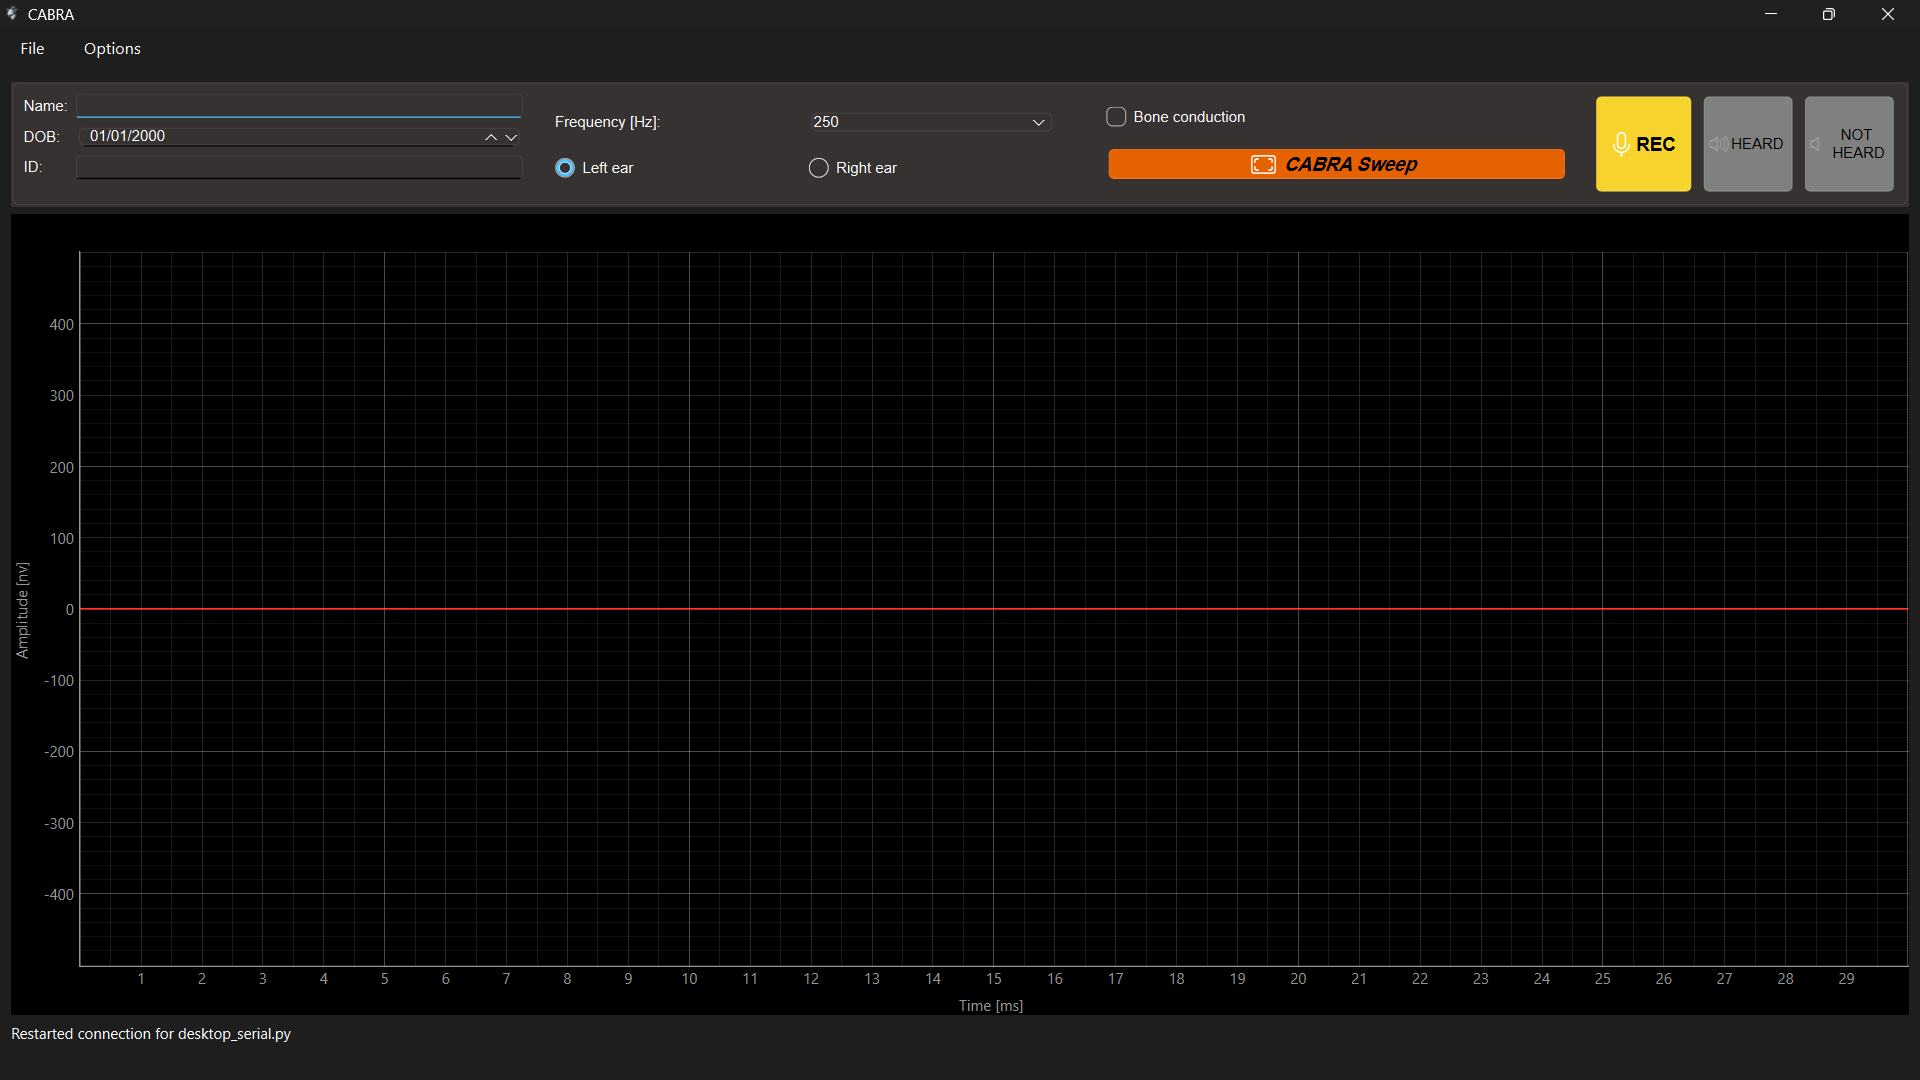
\includegraphics[width=1\linewidth]{figuras/UI-general-view.png}
    \caption{Interfaz gráfica del cliente de escritorio.}
    \label{fig:UI-general-view}
\end{figure}

\subsection{Usabilidad}

Para mejorar la usabilidad del dispositivo, se implementaron una serie de características que facilitan su uso.
Entre ellas, se destaca la posibilidad de guardar y cargar configuraciones previas, la visualización de las ondas
obtenidas en cada prueba, la posibilidad de realizar una audiometría completa y la inclusión de un sistema experto
que sugiere si el paciente percibió o no el estímulo sonoro.
El algoritmo CABRA \textit{Sweep} permite realizar una audiometría completa en un solo paso, lo que facilita la
realización de la prueba evitando confusiones por parte del usuario.
De esta manera, el usuario sólo debe concentrarse en interpretar los resultados obtenidos, sin necesidad de realizar
ajustes manuales de la configuración.
Además, se incluyeron mensajes de error y advertencia que guían al usuario en el uso del dispositivo.
Entre ellos:

\begin{itemize}
    \item Si el dispositivo se desconecta, se muestra un mensaje de error y se detiene la prueba.
    \item Si las lecturas obtenidas no cumplen con los criterios de amplitud, se informa al usuario y se detiene la
    prueba
    \item Si ocurre algún error en la transmisión de datos, se muestra un mensaje de advertencia y se detiene la prueba
\end{itemize}

Desde el hardware, por diseño, se evitó la necesidad de calibración, ya que se utilizó un potenciómetro para ajustar la
ganancia del último divisor resistivo.
La alimentación es provista por dos pilas de 3.7V, que se pueden reemplazar o recargar fácilmente.
Las únicas dos fichas externas de conexión del dispositivo son un puerto USB y un jack de 3.5mm, fácilmente
diferenciables y accesibles, las cuales están dispuestas en extremos opuestos de la carcasa.
Las fichas hembra de los cables de electrodos son de colores distintos, lo que facilita su conexión.
Todos los demás componentes son inaccesibles si la carcasa se encuentra cerrada, pero son a su vez fácilmente
reemplazable si se remueve la tapa.
El dispositivo es portátil y su tamaño es reducido, lo que facilita su transporte y almacenamiento.

\subsection{Análisis de riesgo}

Se identificaron los siguientes riesgos asociados al uso del dispositivo:

\begin{table}[H]
    \centering
    \begin{table}[H]
        \centering
        \caption{\small Tabla de análisis de riesgo.}
        \hspace*{-2cm}
        \begin{tabular}
        {|>{\centering\arraybackslash}p{1.8cm}|
            >{\centering\arraybackslash}p{1.8cm}|
            >{\centering\arraybackslash}p{1.8cm}|
            >{\centering\arraybackslash}p{1.8cm}|
            >{\centering\arraybackslash}p{1.8cm}|
            >{\centering\arraybackslash}p{1.8cm}|
            >{\centering\arraybackslash}p{1.8cm}|
            >{\centering\arraybackslash}p{1.8cm}|}
            \hline
            \textbf{\small Riesgo}
            & \textbf{\small Causa}
            & \textbf{\small Efecto}
            & \textbf{\small Probable}
            & \textbf{\small Severidad}
            & \textbf{\small Control Actual}
            & \textbf{\small Evaluacion}
            & \textbf{\small Análisis}
            \\
            \hline
            \small Error de conexión
            & \small Desconexión del dispositivo
            & \small Interrupción de la prueba
            & \small Media
            & \small Grave
            & \small Uso de cable USB reforzado
            & \small Aceptable
            & \small Utilizar cable más robustos (ej.: USB tipo C)
            \\
            \hline
            \small Colocación incorrecta de los electrodos
            & \small Conexión incorrecta de los electrodos
            & \small Resultados erróneos
            & \small Media
            & \small Grave
            & \small Manual de usuario detallado
            & \small Aceptable
            & \small Capacitación del usuario
            \\
            \hline
            \small Conexión de electrodos bien colocados a entradas incorrectas
            & \small Confusión en la colocación de fichas hembra de cable paciente
            & \small Resultados erróneos
            & \small Baja
            & \small Grave
            & \small Colores distintos en fichas hembra
            & \small Aceptable
            & \small Instrucciones claras en manual de usuario
            \\
            \hline
            \small Falla en la calibración de volumen & \small Ajuste incorrecto del volumen a 0 [dBHL] para la frecuencia base
            & \small Resultados erróneos, lesión auditiva
            & \small Baja
            & \small Grave
            & \small Calibración de fábrica
            & \small Inaceptable
            & \small Implementar una
            \small interfaz de calibración de volumen
            \\
            \hline
            \small Descarga eléctrica
            & \small Cortocircuito en la placa de preacondicionamiento
            & \small Lesión física
            & \small Baja
            & \small Grave
            & \small Aislamiento del circuito dentro de la carcasa
            & \small Inaceptable
            & \small Verificar aislamiento de componentes
            \\
            \hline
        \end{tabular}
        \label{tab:analisis_riesgo}
    \end{table}
\end{table}

\label{pruebas}

Para verificar la funcionalidad del equipo, se llevaron a cabo una serie de pruebas ante diferentes condiciones de
operación:

\begin{itemize}
    \item Desconexión y reconexión por USB del dispositivo
    \item Muestreo con el microcontrolador desconectado de la placa de preacondicionamiento
    \item Muestreo con el paciente no conectado
    \item Prueba con el paciente conectado, sin estímulo sonoro
    \item Prueba con el paciente conectado, con estímulo sonoro reportado como perceptible
    \item Simulación de una audiometría completa, con umbrales auditivos creados con números aleatorios
\end{itemize}

Debido al tiempo que se requiere para realizar una prueba completa dado el rendimiento del dispositivo, resultó
implausible de llevarse a cabo fuera de la simulación planteada.
